\documentclass[11pt,a4paper,onecolumn,final]{article}

%OT1 is the default font encoding of memoir class
%It is generally advised to put it before inputenc
%\usepackage{kerkis}
\usepackage[T1]{fontenc}

%Input encoding for typing directly Greek characters
%Other values for the option: latin1, ascii, ansinew
%It is generally advised to put it before babel
\usepackage[utf8]{inputenc}

%MAIN Language the LAST one
\usepackage[greek,english]{babel}

%\usepackage{kerkis}

%The teubner package extends the facilities offered by the CB Greek fonts
%NOTE: This includes also the graphicx package!
%NOTE: When the teubner package is loaded, command \cap (denoting set intersection) is overwritten
%NOTE: TEUBNER.STY FILE HAS BEEN CHANGED A BIT IN LINES 255-257 WITH 3 REPLACEMENTS \cap -> \capt
\usepackage{teubner}

%Package for displaying math
\usepackage{amsmath}

%Loading a superset of amsfonts
\usepackage{amssymb}

%Provides an enhanced version of \newtheorem
%1.Defines * for unnumbered environments
%2.Defines a proof environment
%3.Defines plain, definition, and remark theorem styles
\usepackage{amsthm}

%Allows text in eps files to be replaced with LATEX symbols
\usepackage{psfrag}

%An extension of the cite package, compatible with the IEEEtranN bibliography style
\usepackage[numbers,sort&compress]{natbib}

\makeatletter\let\c@lofdepth\relax\let\c@lotdepth\relax\makeatother
\usepackage[small,bf,tight]{subfigure}

%Math symbols of the dsfont style. Enables the use of \mathds{}
\usepackage{dsfont}

%Defines several symbols in text mode (e.g. the \textreferencemark for use in the itemize environment)
\usepackage{textcomp}

%Enables the Ralph Smith's Formal Script font in math mode via the \mathscr{} command
\usepackage{mathrsfs}

\usepackage{geometry}
%PDF VIEW
\geometry{total={210mm,297mm},left=25mm,right=25mm,bindingoffset=0mm, top=25mm,bottom=25mm}
%PRINT
%\geometry{total={210mm,297mm},left=20mm,right=20mm,bindingoffset=10mm, top=25mm,bottom=25mm}

\usepackage[breaklinks=true,colorlinks=true,
%linkcolor=blue,urlcolor=blue,citecolor=blue,% PDF VIEW
linkcolor=black,urlcolor=black,citecolor=black,% PRINT
bookmarks=false,bookmarksopenlevel=2]{hyperref}
\usepackage{bm}

%Convenient language switch
\newcommand{\gr}[1]{\foreignlanguage{greek}{#1}}
\newcommand{\en}[1]{\foreignlanguage{english}{#1}}
\newcommand{\dmin}{d_\text{min}}
\newcommand{\eps}{\varepsilon}

%\newtheorem{definition}{Ορισμός}
\newtheorem{definition}{Definition}
\newtheorem{example}{Example}
\newtheorem{exercise}{Exercise}
%\newtheorem{lemma}{Λήμμα}
\newtheorem{lemma}{Lemma}
%\newtheorem{proof}{Proof}
\newtheorem{notation}{Notation}
\newtheorem{problem}{Problem}
%\newtheorem{proposition}{Πρόταση}
\newtheorem{proposition}{Proposition}
\newtheorem{remark}{Remark}
\newtheorem{solution}{Solution}
\newtheorem{summary}{Summary}
\newcommand{\argmax}{\arg\!\max}
%\addto\captionsgreek{\renewcommand{\chaptername}{Κεφάλαιο}}
%\addto\captionsgreek{\renewcommand{\tablename}{Πίνακας }}
%\addto\captionsgreek{\renewcommand{\proofname}{Απόδειξη }}
\setlength{\parindent}{0pt}
\setcounter{section}{-1}
\graphicspath{{./media/}}

\makeatletter
%\renewcommand{\fnum@figure}{Σχήμα \thefigure}
%\renewcommand{\fnum@table}{Πίνακας \thetable}
\makeatother
\begin{document}

%COVER PAGE%%%%%%%%%%%%%%%%%%%%%%%%%%%%%%%%%%%%%%%%%%%%%%%%%%%%%%%%%%%%%%%%%%%%%
\thispagestyle{empty}
{\sffamily\centering\Large

\vspace{\fill}

{\Large Aristotle University of Thessaloniki\\
Department of Electrical and Computer Engineering\\
Telecommunications Division}\\[0.5cm]


\vspace{2.0cm}

{\LARGE Ioannis Dimoulios 10641 \\
        Dimitrios Diakoloukas 10642}

\vspace{3.5cm}


{\LARGE Communication Systems II}\\[1em]

{\Large Constellation Design for Simultaneous  Wireless Information and Power Transfer (SWIPT)}

\vspace{3.5cm}

%\vspace{\fill}

%
}
%%COVER PAGE%%%%%%%%%%%%%%%%%%%%%%%%%%%%%%%%%%%%%%%%%%%%%%%%%%%%%%%%%%%%%%%%%%%%%

\newpage


%ABSTRACT%%%%%%%%%%%%%%%%%%%%%%%%%%%%%%%%%%%%%%%%%%%%%%%%%%%%%%%%%%%%%%%%%%%%%%%
%\chapter*{Abstract}
%\en{In this paper...}
%ABSTRACT%%%%%%%%%%%%%%%%%%%%%%%%%%%%%%%%%%%%%%%%%%%%%%%%%%%%%%%%%%%%%%%%%%%%%%%

\newpage

%\tableofcontents


\section{Introduction}
The task requires the analysis and design of various constellations considering the
balance in simultaneous wireless information and power transfer (SWIPT) systems.
Specifically, the focus is on the relationship between peak-to-average power ratio (PAPR)
and minimum Euclidean distance ($d_{\text{min}}$) in designing optimal constellations for SWIPT and reviewing their performance in terms of symbol error rate (SER).

We examine known modulation schemes such as 16-PAM, 16-PSK, and 16-QAM, as well as the state of the art 16-Circular QAM (CQAM) and 16-Spike QAM (sQAM) as presented in \cite{cqam} and \cite{sqam} respectively. In the final sections of the assignment we propose a new modulation scheme, namely 16-Bee QAM (BQAM), which shows promising results. 

Our approach includes both a theoretical and a simulation analysis. Constellations are represented with simple arrays of complex numbers in Julia with the convention that the first two symbols of the array always have distance \(d_\text{min}\). A more thorough explanation of our software setup is included in the Appendix section.  


\section{PAPR versus Minimum Euclidean Distance}
In what follows the average symbol energy for all the constellations is normalized on \(E_s = 1\). This ensures that the comparisons are fair energy-wise. Moreover, \(M = 16\) is the number of symbols for each constellation. 

\subsection{Theoretical Analysis}
\subsubsection*{16-PAM} 
Assume that the energy of the main pulse of the PAM is \(E_g\). It is well known that 
\begin{equation}
    E_g = \frac{3E_s }{M^2 - 1} = 0.0118. 
\end{equation}
Then, given that the symbol with the highest energy, i.e. the symbol furthest from the origin has coordinates 
\begin{equation}
    x_M = \left\{(M-1)\sqrt{E_g}\right\}, 
\end{equation}
we can calculate PAPR as follows 
\begin{equation}
    \text{PAPR}_\text{PAM} = \frac{|x_M|^2}{E_s} = 2.647.
\end{equation}
As far as the minimum euclidean distance is concerned, we have
\begin{equation}
    d_\text{min} = 2\sqrt{E_g} = 0.217.
\end{equation}

\begin{figure}[h]
    \centering
    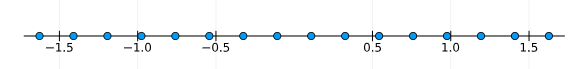
\includegraphics[scale=0.7]{16pam.png}
    \caption{16-PAM constellation diagram}
\end{figure}

\newpage

\subsubsection*{16-PSK}
The symbols of PSK have coordinates 
\begin{equation}
    x_i = \left\{ \sqrt{E_s}\cos \theta_i, \sqrt{E_s} \sin \theta_i \right\}
\end{equation}
where \(\theta_i = \dfrac{2\pi (i-1) }{M}\) for all \(i = 1, \ldots, M\). Hence for all \(i\), we have 
\begin{equation}
    E_i = |x_i|^2 = \sqrt{\cos ^2 \theta_i + \sin ^2 \theta_i} = 1,
\end{equation}
which in turn means \(E_\text{max}\) = 1 and
\begin{equation}
    \text{PAPR}_\text{PSK} = \frac{E_\text{max}}{E_s } = 1. 
\end{equation}
It also follows from simple trigonometric calculations that 
\begin{equation}
    d_\text{min} = 2\sqrt{E_s}\sin \frac{\pi}{M } = 0.390. 
\end{equation}

\begin{figure}[h]
    \centering
    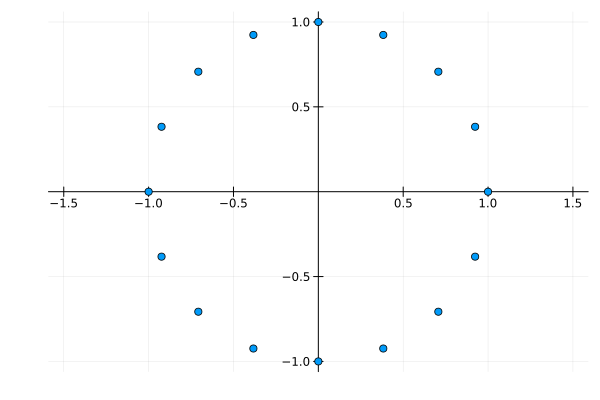
\includegraphics[scale=0.7]{16psk.png}
    \caption{16-PSK constellation diagram}
\end{figure}

\subsubsection*{16-QAM}
\(M\)-QAM is essentially the composition of two orthogonal \(\sqrt{M}\)-PAM constellations representing the I/Q components of the constellation. The energy is equally shared between each component; hence 
\begin{equation}
    E_s = 2E_{s\left(\sqrt{M}-\text{PAM}\right)}
\end{equation}
and if \(E_g\) is the energy of the main pulse of each \(\sqrt{M}\)-PAM component we have
\begin{equation}
    E_g = \dfrac{3E_{s\left(\sqrt{M}-\text{PAM}\right)}
}{\sqrt{M}^2 - 1} = \dfrac{1.5E_s }{M - 1} = 0.1.
\end{equation}
Then the coordinates of the symbol with the highest energy are 
\begin{equation}
    x_M = \left\{ \left(\sqrt{M} - 1\right)\sqrt{E_g}, \left(\sqrt{M} - 1\right)\sqrt{E_g} \right\}. 
\end{equation}
Now, we can calculate 
\begin{equation}
    \text{PAPR}_\text{QAM} = \frac{|x_M|^2 }{E_s } = 0.1\cdot 2 \cdot 3^2 = 1.8.
\end{equation}
On the other hand 
\begin{equation}
    d_\text{min} = 2\sqrt{E_g} = 0.632.
\end{equation}
\begin{figure}[h]
    \centering
    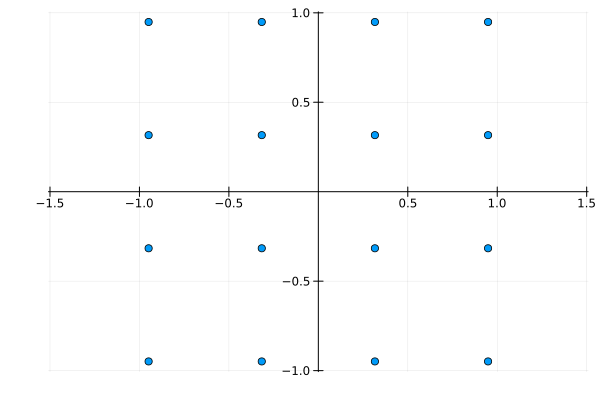
\includegraphics[scale=0.7]{16qam.png}
    \caption{16-QAM constellation diagram}
\end{figure}

\subsubsection*{16-CQAM}
According to the algorithm provided \cite{cqam} we initialize CQAM as a function of two parameters: 
\begin{itemize}
    \item \(N\), the number of circles of the constellation and
    \item \(d_\text{min}\), the minimum euclidean distance, from which we can directly calculate the radius of the first circle. 
\end{itemize}
Each circle must contain \(n = M \div N \) symbols. Indeed, the first radius is 
\begin{equation}
    R_1 = \frac{d_\text{min} }{2\sin \frac{\pi}{ n}}.
\end{equation}\\ 
Next, we create the first circle with \(n \) symbols such that adjacent symbols are distanced at \(d_\text{min}\). 

The next \(N-2\) circles are formed with \(n\) with the minimum possible radius such that the \(d_\text{min}\) condition is not violated. 

The remaining energy is then used to form the last circle with radius \(R_N > R_j\) \\ for all \(j \in 1,\ldots , N-1\).

Hence, considering that the symbols carrying the maximum energy are those of the last circle we can calculate,  
\begin{equation}
    \text{PAPR}_\text{CQAM} = \frac{R_N^2}{E_s } = R_N^2. 
\end{equation}
In order to create these constellations on software, we used rotating vectors of modulus \(d_\text{min}\) to form equilateral triangles on the first \(N-1\) circles. The results are presented in the diagram below. 

\begin{figure}[h]
    \centering
    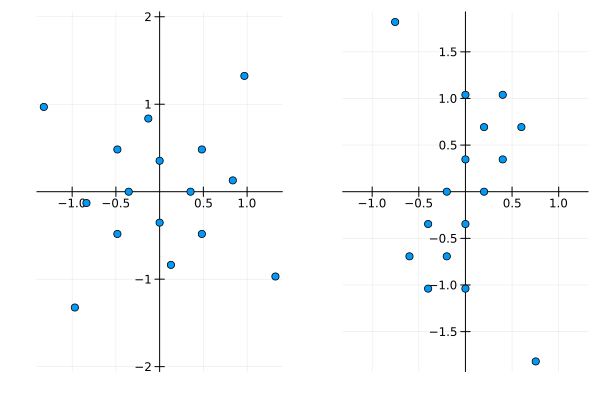
\includegraphics[scale=0.7]{16cqam_dual.png}
    \caption{16-CQAM constellations, a) with \(N=4\), \(\dmin = 0.5\)} and b) with \(N=8\), \(\dmin = 0.4\)
\end{figure}

\subsection{Simulation Results}
For PAPR calculations, we used the normalized average \(E_s = 1\) for each constellation and found the symbol with maximum energy by means of linear search. 

For \(\dmin \) calculations, we made sure we adhered to the convention stated in the introduction, namely that the first two symbols of the constellation are distanced at \(\dmin\). 

The simulations are therefore summarized in the following figure. 

\newpage
\begin{figure}[h]
    \centering
    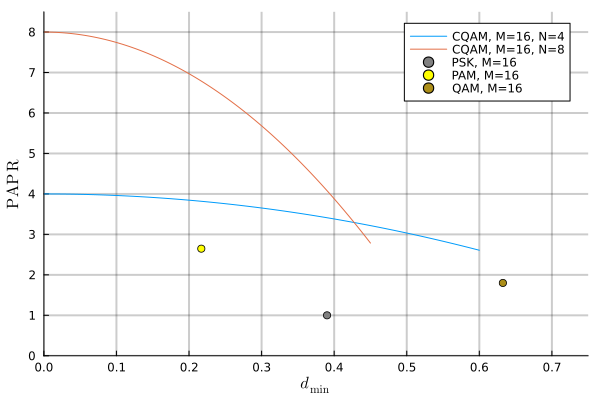
\includegraphics[scale=0.7]{ex1_sim.png}
    \caption{PAPR versus \(\dmin \) plot for various modulation schemes}
\end{figure}

Notice that the PSK point differs from the one presented in \cite{cqam}. Additionally, there is a slight variation for both the CQAM curves compared to \cite{cqam}. 

\subsection{Detailed Review of Calculations}

\subsubsection*{16-PAM}
\begin{enumerate}
    \item \textbf{Power Vector Calculation:}\\
    For 16-PAM, we calculate the power of each symbol. The symbols are spaced equally, and the power of each symbol is determined by squaring the difference between the symbol position and the center point of the constellation. This results in a power vector that contains the power values for all 16 symbols.
    \item \textbf{Average Power Calculation:}\\
    The total power is obtained by summing all elements in the power vector. The average power is then calculated by dividing this total power by the number of symbols, \(M\).
    \item \textbf{Maximum Power Calculation:}\\
    The maximum power in 16-PAM is determined by the power of the outermost symbol, which is the symbol with the highest amplitude. This is given by the square of \((M - 1)\).
    \item \textbf{PAPR Calculation:}\\
    The Peak-to-Average Power Ratio (PAPR) is calculated by dividing the maximum power by the average power.
    \item \textbf{Minimum Euclidean Distance (\(d_{\text{min}}\)) Calculation:}\\
    The minimum Euclidean distance is calculated from the energy per symbol. The energy per symbol is the reciprocal of the average power. The minimum distance between adjacent symbols is then \(2 \sqrt{\text{energy per symbol}}\).
\end{enumerate}

\subsubsection*{16-PSK}
\begin{enumerate}
    \item \textbf{PAPR Calculation:}\\
    For PSK modulation, the PAPR is always 1 because all symbols have the same amplitude. This results in a constant envelope signal.
    \item \textbf{Minimum Euclidean Distance (\(d_{\text{min}}\)) Calculation:}\\
    The minimum Euclidean distance for PSK is calculated based on the radius of the circle on which the symbols are placed. The distance between adjacent symbols on the circle is determined by the angle between them, which is \(2 \pi / M\). The formula used is \(2 \times \text{radius} \times \sin(\pi / M)\).
\end{enumerate}

\subsubsection*{16-QAM}
\begin{enumerate}
    \item \textbf{Power Vector Calculation:}\\
    For 16-QAM, the symbols are arranged in a square grid. The power of each symbol is calculated by summing the squares of its x and y coordinates. This results in a power vector that contains the power values for all symbols in the constellation.
    \item \textbf{Average Power Calculation:}\\
    The total power is obtained by summing all elements in the power vector. The average power is then calculated by dividing this total power by the number of symbols, \(M\).
    \item \textbf{Maximum Power Calculation:}\\
    The maximum power in 16-QAM is determined by finding the maximum value in the power vector. This corresponds to the symbol with the highest combined x and y coordinates.
    \item \textbf{PAPR Calculation:}\\
    The PAPR is calculated by dividing the maximum power by the average power.
\end{enumerate}

\subsubsection*{16-CQAM}
\begin{enumerate}
    \item \textbf{Radius Calculations for CQAM:}\\
    In CQAM, symbols are placed on concentric circles. The radii of these circles are calculated iteratively to ensure that the minimum distance between symbols is maintained. The first radius is determined based on the minimum distance divided by \(2 \sin(\pi / n)\), where \(n\) is the number of symbols per circle. Subsequent radii are calculated to maintain the minimum distance constraint.
    \item \textbf{PAPR Calculation:}\\
    The PAPR for CQAM is determined by the radius of the outermost circle. The maximum power is given by the square of the radius of this circle. The average power is calculated by averaging the power of all symbols, and the PAPR is then the maximum power divided by the average power.
\end{enumerate}
% Unfortunately, we could not get the exact results demonstrated in the paper. 

\section{SER versus Harvested Energy and SNR}
Our goal is to study the SER as a function of both the normalized harvested energy and the Signal to Noise Ratio (SNR). Note that we define SNR as 
\begin{equation}
    \text{SNR} = \frac{E_b}{N_0} = \frac{E_s }{N_0 \log_2 M}. 
\end{equation}
To that end, we have made a few assumptions regarding the receiver. Firstly, the energy is harvested and then the noise is added. Moreover, the demodulator is aware of the energy transfer the adjusts the constellation accordingly. Lastly, we work in a very high SNR environment.

\subsection{Theoretical Analysis}
Harvesting a portion of the energy of a transmitted symbol corresponds to the following transform of the symbol in the constellation space; if \(x\) is the transmitted symbol represented by a complex number, \(\eps(x)\) is the amount of energy harvested, and \(\delta^+ = \max(0, \delta)\), then 
\begin{equation}
    x = re^{i\theta} \mapsto \sqrt{(r^2 - \eps(x))^+} e^{i\theta}. 
\end{equation}
Of course, this transform applied to symbols with \(\dmin\) distance generates a new and reduced minimum distance \(\dmin '\) for the constellation. In that spirit and taking into consideration the high SNR environment we approximate the SER of a symbol by assuming that it can only be mistaken for a ``neighbor'', i.e. another symbol which is \(\dmin '\)  away. In order to account for the complex constellation geometries generated by the energy harvest transform, we extend the definition of a ``neighbor'' by adding a small tolerance of \(\dfrac{\dmin '}{c\cdot\text{SNR}}\), where \(c > 1\) is a positive constant. For the sake of this assignment we pick \(c = 5\). 

Formally, we define the set of neighbors of a symbol in the transformed constellation as 
\begin{equation}
    G(i) = \left\{ x_j \mid |x_i - x_j| \leq \dmin ' \left(1 + \frac{1}{c \cdot \text{SNR}}\right) \right\}, 
\end{equation}
where \(\{x_k\}_{1 \leq k \leq M}\) is the set of the symbols of the transformed constellation.

However, we are mostly interested in the cardinality of \(G\); hence, define 
\begin{equation}
    v(i) = |G(i)| 
\end{equation}
for all \(1 \leq i \leq M\) to be the number of neighbors of the symbol \(x_i\). 
Note that \(v(i)\) changes as \(\eps(x)\) increases. 

For example, consider a 16-PAM constellation and let \(\eps(x_i) = \eps\) for all \(1 \leq i \leq 16\). Then, if 
\begin{itemize}
    \item \(\eps = 0\), \(\dmin = 0.217\) and \(v(16) = 1\), 
    \item \(\eps = 0.5\), \(\dmin ' = 0\) and \(v(16) = 0\). 
\end{itemize}
This volatility on the values of \(v(i)\) makes the construction of a formula for SER as a function of \(\eps\) extremely hard. Luckily, we can bypass this by calculating for each \(\eps\) the new \(\dmin '\) and the array of \(v(i)\)s. 

We proceed by providing constellation specific insights for SER calculation. 

\subsubsection*{16-PAM}
It is straightforward that
\begin{align}
    \text{SER}_j &= v(j)Q\left(\sqrt{\frac{6E_s }{(M^2 - 1) N_0}}\right) = v(j)Q\left(\frac{\dmin ' }{\sqrt{2N_0}}\right) \\
    \text{SER}_\text{PAM} &= \frac{1}{M }\sum_{j = 1}^{M } \text{SER}_j = \frac{1}{M }\sum_{j = 1}^{M }v(j)Q\left(\frac{\dmin ' }{\sqrt{2N_0}}\right)
\end{align}
For \(\eps = 0\), this becomes 
\begin{equation}
    \text{SER} = Q\left(\sqrt{\frac{6E_s }{(M^2 - 1) N_0}}\right) = Q\left(\sqrt{\frac{6\log_2 M \cdot\text{SNR}}{(M^2 - 1)}}\right).
\end{equation}

\subsubsection*{16-QAM}
When \(\eps > 0\) the constellation loses its straight line grid structure, but we can still approximate it as such. Hence, by considering the I/Q decomposition in two orthogonal 4-PAM's we get the estimation
\begin{align}
    \text{SER}_j &\approx 1 - (1 - \text{SER}_{Ij})(1 - \text{SER}_{Qj}) \\
        &=  1 - \left[1 - v_I(j)Q\left(\frac{\dmin ' }{\sqrt{2N_0}}\right)\right]\left[1 - v_Q(j)Q\left(\frac{\dmin ' }{\sqrt{2N_0}}\right)\right],
\end{align}
where \(v_I(\cdot)\) and \(v_Q(\cdot)\) represent the number of neighbors on the I and Q component respectively. By taking the mean over all \(\text{SER}_j\), we can find a good approximation for \(\text{SER}_\text{QAM}\). 

For \(\eps = 0\), this becomes
\begin{equation}
    \text{SER} = 1 - \left[1 - Q\left(\sqrt{\frac{1.5\log_2 M \cdot \text{SNR}}{M - 1}}\right)\right]^2
\end{equation}
as the energy is equally distributed among the I and Q components and we have \(\sqrt{M}\) instead of \(M\). 
\begin{figure}[h]
    \centering
    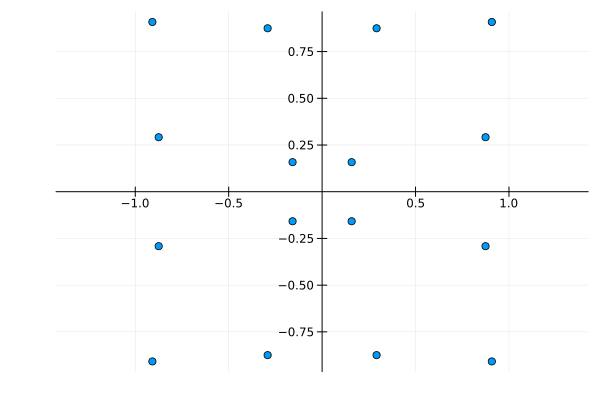
\includegraphics[scale=0.6]{16qam_e015.png}
    \caption{16-QAM constellation diagram with \(\eps = 0.15\)}
\end{figure}

\subsubsection*{16-CQAM}
Assume the variables introduced in the former analysis in section 1 are the same. According to \cite{cqam}, we can approximate the error rate as follows
\begin{equation}
    \text{SER}_\text{CQAM} = \frac{1}{N} \sum_{j = 1}^{N }v(i)Q\left(\sqrt{\text{SNR} \sin \frac{\pi}{n}\left(\sqrt{R_j^2 - \eps }\right)^+}\right). 
\end{equation}

\subsubsection*{16-sQAM}
We will use the configuration from \cite{sqam} with \(4\) spikes. On this constellation it only makes sense to harvest energy from the symbols corresponding to the spikes. Otherwise, the reason of existence of the spikes would be neutralized. Of course, it will have to be normalized to match the total harvested energy of the other constellations with constant \(\eps \) across all their symbols. For clarity, this means if we have \(\ell\) spikes and \(\eps \) was the constant harvested energy of every single symbol on the rest of the constellations, then, 
\begin{equation}
    \eps ' = \eps(\text{spike}) = \frac{\eps M }{\ell}. 
\end{equation}
This is shown on the constellation diagram below. Note that the symbols not corresponding to spikes are identical, while energy has only be harvested from the spiked symbols. 

For the theoretical calculation of the symbol error probability, we emply the approximation outlined in \cite{sqam}. However we first need to calculate the PAPR. This is straight-forward as given the \(\dmin\), we can find the PAPR of the unnormalized constellation corresponding to that minimum distance by reverse engineering the process in the theoretical analysis of the first section. This is essentially the energy of 4 corner symbols, which will also be spiked. 

To achieve this we add the remaining energy to those corner elements to reach average energy \(E_s = 1\) and then the \(\text{PAPR} = |x_M|^2\), where \(x_M\) is one of the corner symbols. Then, we define the following constants: 
\begin{align}
    k &= \left(\frac{(2(M - 1)}{3}\right)^{-(1/2)} \\
    \gamma &= \frac{M - \ell \cdot \text{PAPR}}{M - \ell} \\
    D_\text{mid} &= k\sqrt{2M - 8\sqrt{M} + 8}. 
\end{align}
Now we are ready to calculate the SER. Indeed, 
\begin{align}
    \text{SER}_\text{QAM}^\gamma &= 1 - \left[1 - Q\left(\sqrt{\frac{1.5\log_2 M \cdot \text{SNR}}{M - 1}\gamma}\right)\right]^2, \\
    \text{SER}_\text{QAM}^\text{max} &= Q\left(\frac{|x_M| - D_\text{mid} - \eps '}{\sqrt{2N_0}}\right),
\end{align}
Note the normalizing constant \(\gamma \), as well as the extraction of energy from the spike symbols. Then, 
\begin{equation}
    \text{SER}_\text{sQAM} = \frac{M - \ell}{M }\text{SER}_\text{QAM}^\gamma + \frac{\ell }{M }\text{SER}_\text{QAM}^\text{max}
\end{equation}
\begin{figure}[h]
    \centering
    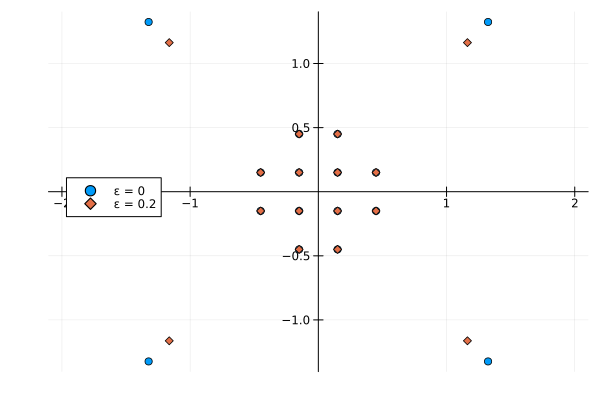
\includegraphics[scale=0.6]{16sqam_both0and02.png}
    \caption{16-sQAM constellation diagram of \(\dmin = 0.3\) with \(\eps = 0\) and \(\eps = 0.2\)}
\end{figure}

\subsection{Simulation Results}
We have devised a Monte-Carlo simulation environment where we repeat the same experiment for a specific number of attempts and log the ratio of the errors to the number of the attempts in each of the two cases. 

\subsubsection*{SER over \(\eps(x)\)}
The results of SER over \(\eps(x)\) simulation are summarized in the following graph. 

\begin{figure}[h]
    \centering
    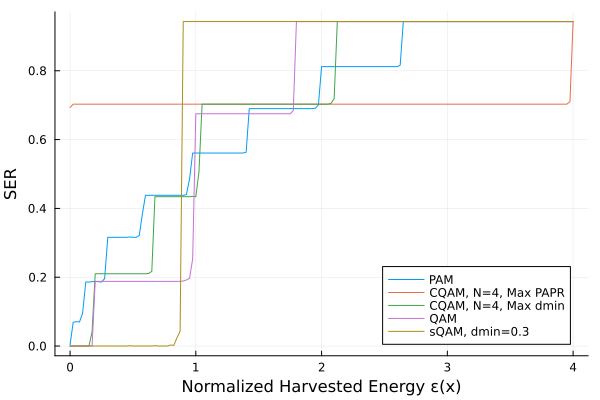
\includegraphics[scale=0.59]{ex2_a.png}
    \caption{SER as a function of \(\eps(x)\) simulation graph}
\end{figure}
Excluding CQAM, the results are identical to those presented in \cite{cqam}. 

Regarding sQAM, it outperforms all other modulation schemes up to the point that the spikes are completely degraded to the origin. 

\subsubsection*{SER over SNR}
The results of SER over SNR simulation are summarized in the following graph.  
\begin{figure}[h]
    \centering
    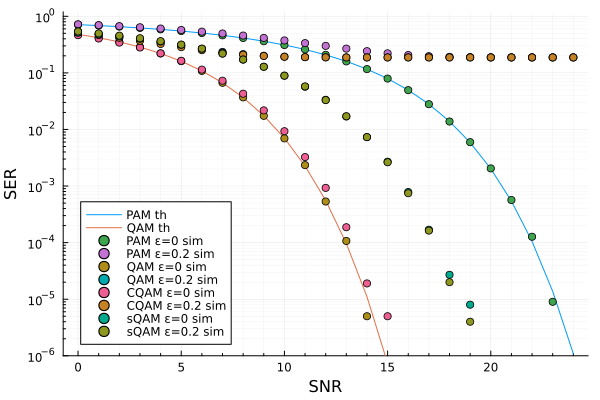
\includegraphics[scale=0.59]{ex2_b.png}
    \caption{SER as a function of SNR simulation graph}
\end{figure}

Note that CQAM with harvesting performance is radically worse to the one in \cite{cqam}. The other curves are very similar though. Moreover, notice that the perfomance of sQAM is not degraded at all despite the harvesting. This is to be expected when harvesting only from the spikes in a very high SNR environment. 

\section{16-Bee QAM (16-BQAM)}
BQAM is a new modulation scheme optimized for SWIPT drawing inspiration from both CQAM and sQAM. 
\begin{figure}[h]
    \centering
    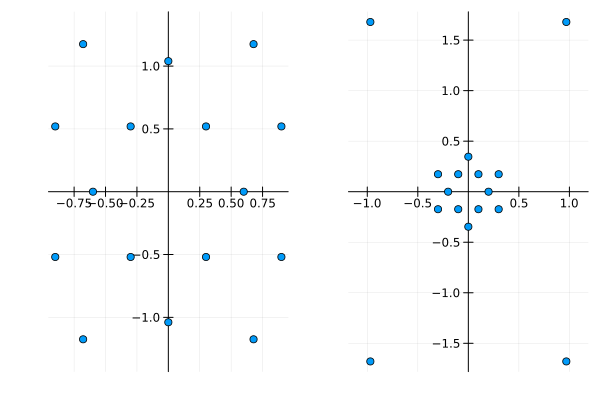
\includegraphics[scale=0.57]{bqam_both.png}
    \caption{16-BQAM constellations, a) with \(\dmin = 0.6\) and b) with \(\dmin = 0.2\)}
\end{figure}

It consists of two 6-PSKs such that the distance between any two of their 12 symbols in total is \(\dmin\). The remaining energy is used for the other 4 symbols, which form a 4-PSK with the maximal energy. The idea can be generalized for higher order modulations with \(M = 4^k\) symbols, such that \(M \equiv 4 \pmod 6\) with appropriate restrictions for \(\dmin\). 

We now repeat our former simulation analysis, but this time we include BQAM. 
\begin{figure}[h]
    \centering
    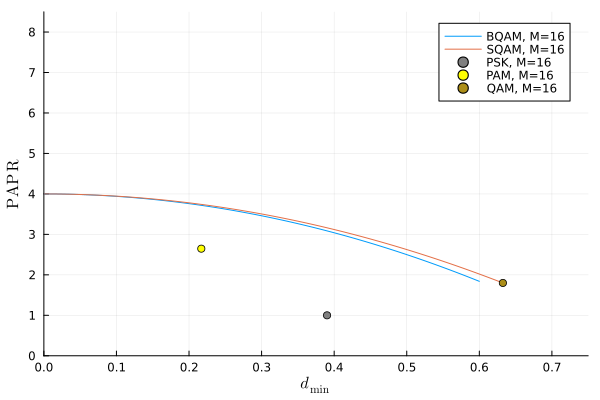
\includegraphics[scale=0.58]{bqam_papr_dmin.png}
    \caption{PAPR over \(\dmin\) plot for BQAM}
\end{figure}

For all possible \(\dmin\) the PAPRs of BQAM and sQAM are almost identical. 

\begin{figure}[h]
    \centering
    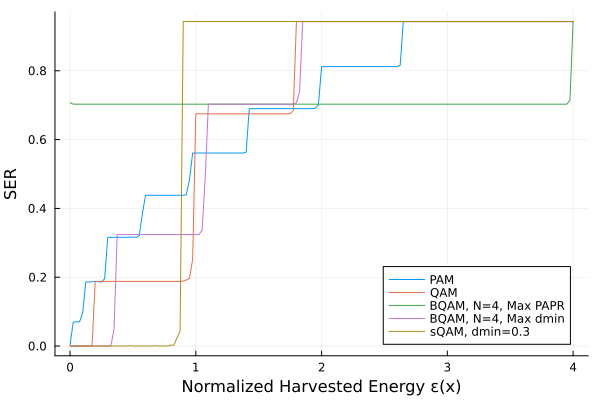
\includegraphics[scale=0.58]{bqam_ex2_a.png}
    \caption{SER as function of \(\eps(x)\) graph with BQAM included}
\end{figure}
It is apparent that a tradeoff between \(\dmin \) and PAPR can be made such that the performance of QAM is matched. Note that we are not harvesting energy exclusively on the spikes of BQAM; hence, the difference with sQAM which does exactly that. 

\begin{figure}[h]
    \centering
    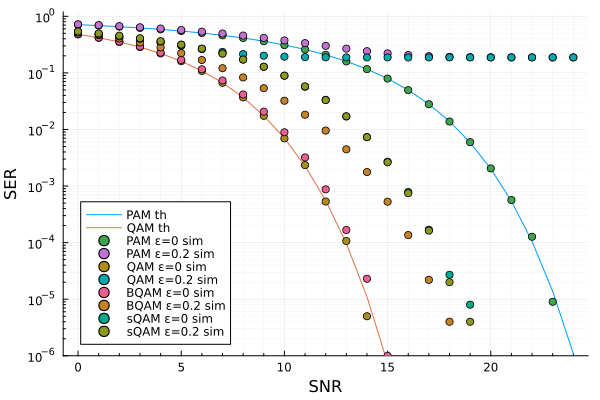
\includegraphics[scale=0.58]{bqam_ex2_b.png}
    \caption{SER as function of \(\eps(x)\) graph with BQAM included}
\end{figure}
Note that BQAM has almost identical SER with QAM without energy harvesting. On the other hand it is cleary superior to all other modulation schemes including sQAM when energy harvesting is taken into account.  

In conclusion, we have shown that in simulations BQAM is indeed better that other known modulation schemes. 
In future iterations we plan to perform a theoretical analysis for this constellation and further optimize it. 

% BQAM outperforms all known modulation schemes in simulations. 


\bibliographystyle{IEEEtranN}
\en{\bibliography{sample}}

\end{document}